
%(BEGIN_QUESTION)
% Copyright 2010, Tony R. Kuphaldt, released under the Creative Commons Attribution License (v 1.0)
% This means you may do almost anything with this work of mine, so long as you give me proper credit

\noindent
{\bf Programming Challenge -- Reversing motor restart delay} 

\vskip 10pt

A three-phase electric motor drives an air heat exchanger (radiative cooler) in either direction (forward or reverse), depending on which way operations personnel wish to blow the warm air.  During warm weather, the preferred direction is up, to direct hot air away from process equipment.  During cold weather, the preferred direction is down, to provide warmth in the process equipment area to help guard against liquid-filled pipes and tubes freezing:

$$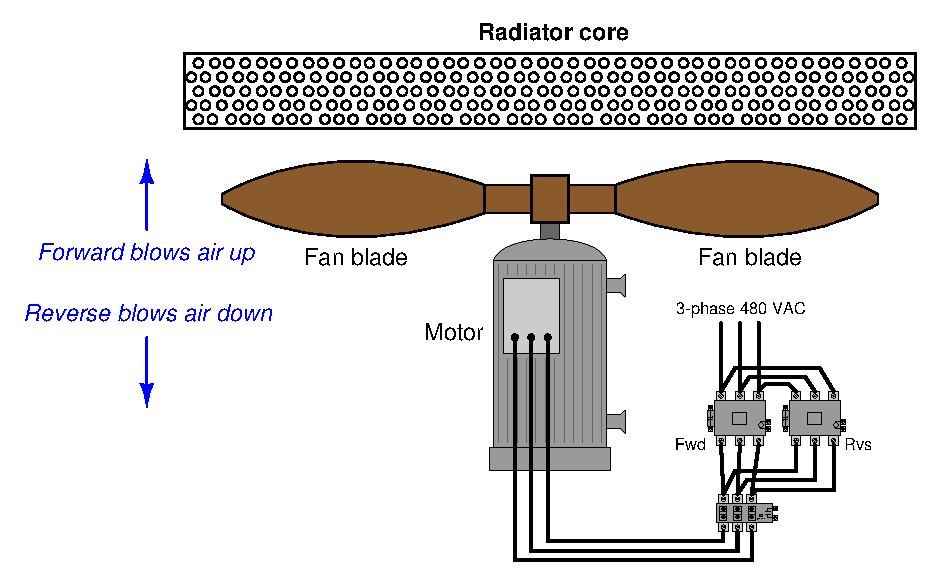
\includegraphics[width=15.5cm]{i02347x01.eps}$$

A reversing start/stop PLC program is easy enough to write, with two momentary-contact ``Start'' pushbuttons (one for Forward, one for Reverse) and one momentary ``Stop'' pushbutton; but what we need here is a reversing program that {\it prevents an immediate re-start of the motor} in the opposite direction following a stop command.  This is because the fan blades have a lot of inertia, and take about 30 seconds to coast to a stop.  This restart lockout timer will prevent someone from trying to reverse the motor's direction before the fan has had a chance to fully stop.

\vskip 10pt

Write a PLC program to provide this forward/reverse/restart lockout functionality.  Assume the use of {\it normally-open} (NO) pushbutton switches for all pushbutton inputs.

\vskip 20pt \vbox{\hrule \hbox{\strut \vrule{} {\bf Suggestions for Socratic discussion} \vrule} \hrule}

\begin{itemize}
\item{} What type of timer instruction is best suited for this application, an {\it on-delay} or an {\it off-delay} timer?
\end{itemize}

\vfil 

\underbar{file i02347}
\eject
%(END_QUESTION)





%(BEGIN_ANSWER)


%(END_ANSWER)





%(BEGIN_NOTES)

I strongly recommend students save all their PLC programs for future reference, commenting them liberally and saving them with special filenames for easy searching at a later date!

\vskip 10pt

I also recommend presenting these programs as problems for students to work on in class for a short time period, then soliciting screenshot submissions from students (on flash drive, email, or some other electronic file transfer method) when that short time is up.  The purpose of this is to get students involved in PLC programming, and also to have them see other students' solutions to the same problem.  These screenshots may be emailed back to students at the conclusion of the day so they have other students' efforts to reference for further study.

\vskip 10pt

When designing a PLC program, a simplifying strategy is to begin simple and then add features, rather than to try to include all features from the very beginning!  In this case, one might start by writing a reversing control program complete with lockouts, but with no timers.  Only after getting this simple program working would the programmer think of trying to add timers to the mix.

%INDEX% PLC, programming challenge: reversing motor restart delay
%INDEX% Process: air-cooled heat exchanger (generic)

%(END_NOTES)


